\subsection{RELIEF: Intelligent Repeaters and Robots for Fast, Reliable, Low-Cost RFID Inventorying \& Localization}

\noindent Context: Project co-financed by EU and Greek National Funds, under the call RESEARCH - CREATE -INNOVATE (project code: T1EDK-03032)\\
\noindent Aristotle University of Thessaloniki, Greece\\
\noindent Duration: 09/2018--09/2021\\

\noindent \textbf{In a nutshell}\\
\noindent \href{http://relief.web.auth.gr/language/en/home/}{\texttt{[Website]}} \href{https://www.facebook.com/ReliefAuth}{\texttt{[fb]}} \href{https://www.youtube.com/@antonidimi/search?query=relief}{\texttt{[Videos]}} \href{https://relief.web.auth.gr/language/en/publications/}{\texttt{[Publications]}} \\


\begin{figure}[H]\centering
  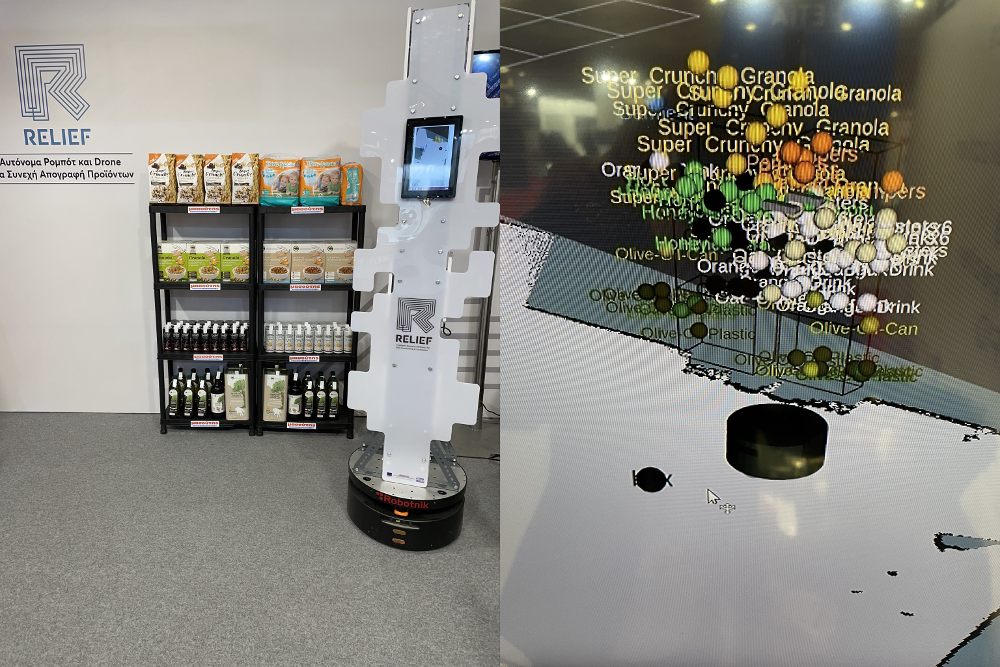
\includegraphics[scale=0.4]{images/relief_1.png}
  \caption{\small Left: RELIEF's heavyweight autonomous ground vehicle at the
           Beyond Expo 2021 and a collection of RFID-tagged typical supermarket
           products. Right: the robot's reconstructed map of
           the products in physical space}
  \label{fig:relief_beyond_1}
\end{figure}

Inventorying and localisation of products in large warehouses is constrained by
the accuracy, precision, and stamina of focus of human-led efforts. If RFID
tags substitute bar codes (optical, remember!), both needs may be fulfilled
with greater accuracy and in less time. If, additionally, robots replace
humans, their time may be liberated for other, more engaging/demanding
activities, and errors may be erased.

The aim of project RELIEF was to provide real-time Simultaneous Robot
Localisation and Mapping of RFID tags in 3D space, with centimeter accuracy. The
means of achieving these goals were three Autonomous Unmanned Robotic Vehicles:

\begin{itemize}
  \item Two
        \href{https://www.youtube.com/watch?v=bo4lMI640DY}{Autonomous Unmanned Ground Vehicles}:
        one modified Yujin Turtlebot 2 (figure \ref{fig:relief_tb_1x4}) and one
        modified Robotnik RB1 (figure \ref{fig:relief_rb1_1x4})
  \item One
        \href{https://www.youtube.com/watch?v=9YpBIaO4tgY}{Autonomous Unmanned Aerial Vehicle}:
        a modified Italdron Evo 4HSE (figure \ref{fig:relief_drone})
\end{itemize}

\noindent Press coverage (Greek only):

\begin{itemize}
  \selectlanguage{greek}
  \singlespacing
  \item \href{https://www.facebook.com/watch/?v=525073015980746}{Έξυπνα ρομπότ - Καλημέρα Θεσσαλονίκη}
  \item \href{https://www.amna.gr/macedonia/article/593568/I-Beyond-40-pigainei-me-Drone-kai-tin-Pliroforia-pio-pera-apo-tin-klironomia-tis-Infosystem}{Η Beyond 4.0 πηγαίνει με Drone και την Πληροφορία πιο πέρα από την κληρονομιά της Infosystem}
  \item \href{https://www.kathimerini.gr/society/561544489/vinteo-k-eikones-apo-to-eggys-mellon-farmaka-apo-drones-parkingk-me-ena-klik-rompot-sta-soyper-market/}{Εικόνες από το εγγύς μέλλον: Φάρμακα από drones, πάρκινγκ με ένα κλικ, ρομπότ στα σούπερ μάρκετ}
  \item \href{https://www.thessnews.gr/reportaz/to-exypno-robot-pou-vriskei-antikeimena-foto-video/}{Το έξυπνο ρομπότ που βρίσκει αντικείμενα}
  \item \href{https://fm100.gr/media/single/o-antonis-dimitrioy-ston-fm100-o-fm100-stin-84i-deth}{Ο ΑΝΤΩΝΗΣ ΔΗΜΗΤΡΙΟΥ ΣΤΟΝ FM100}
  \item \href{https://www.typosthes.gr/thessaloniki/195192_rompot-frida-kanei-bolta-sto-periptero-14-tis-84is-deth-video}{Το ρομπότ FRIDA κάνει βόλτα στο Περίπτερο 14 της 84ης ΔΕΘ!}
  \item \href{https://www.amna.gr/home/videos/391130/Ta-rompot-tou-APTh-stin-84i-DETh}{Τα ρομπότ του ΑΠΘ στην 84η ΔΕΘ}
\end{itemize}


\selectlanguage{english}



Key project aspects are succinctly portrayed through the following videos:

\begin{itemize}
  \singlespacing
  \item \href{https://www.youtube.com/watch?v=bo4lMI640DY}{Autonomous Inventorying and Accurate Real-Time 3D Localization---Library demo}
  \item \href{https://www.facebook.com/watch/?v=960592754415188}{Robots for 24/7 Inventorying and Localization}
  \item \href{https://www.facebook.com/watch/?v=1009958989425825}{Precise Agriculture with Relief Drone and Sustainable Technology}
  \item \href{https://www.facebook.com/watch/?v=1183283855348186}{Experimenting inventorying from above}
  \item \href{https://www.youtube.com/watch?v=9YpBIaO4tgY}{Indoor RFID Drone Inventorying}
\end{itemize}



%\begin{minipage}[t][\textheight]{\textwidth}
\begin{figure}[H]\centering
  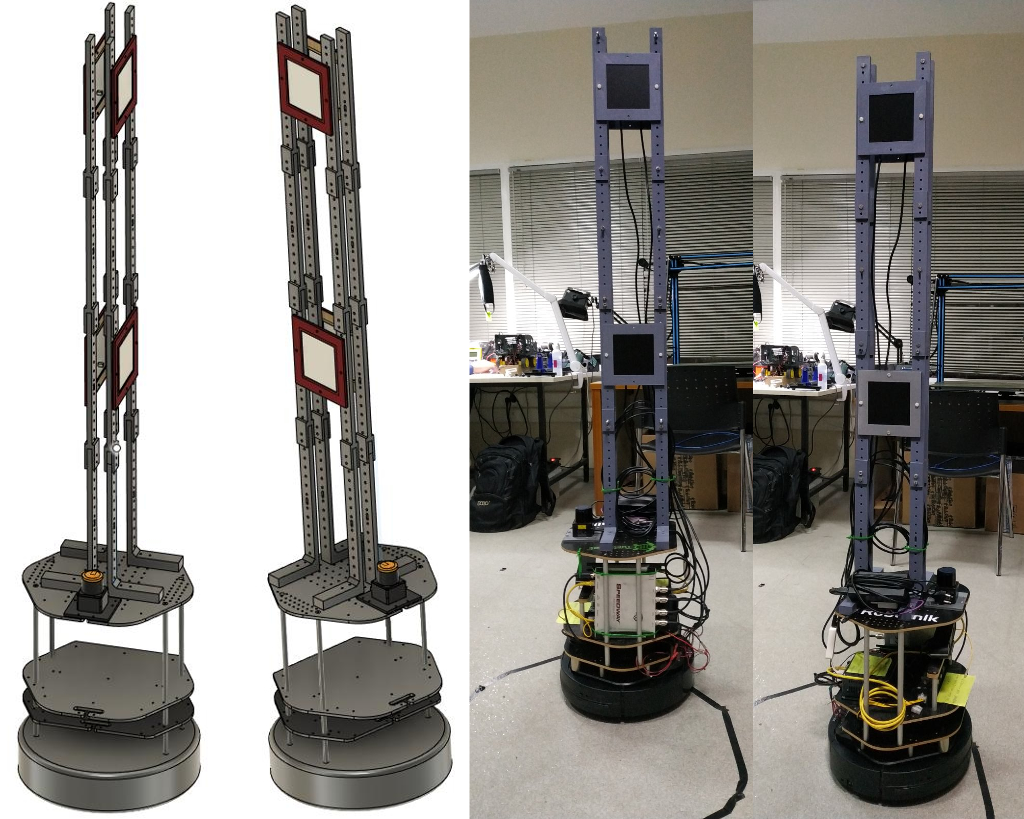
\includegraphics[scale=0.4]{images/relief/tb/tb_1x4.png}
  \caption{\small Views of the design and real (WIP) modified Yujin Turtlebot 2
           robot used as a lightweight autonomous ground vehicle for
           inventorying and 3D localisation of RFID tags. Source: project
           deliverable \#9}
  \label{fig:relief_tb_1x4}
\end{figure}

\vfill

\begin{figure}[H]\centering
  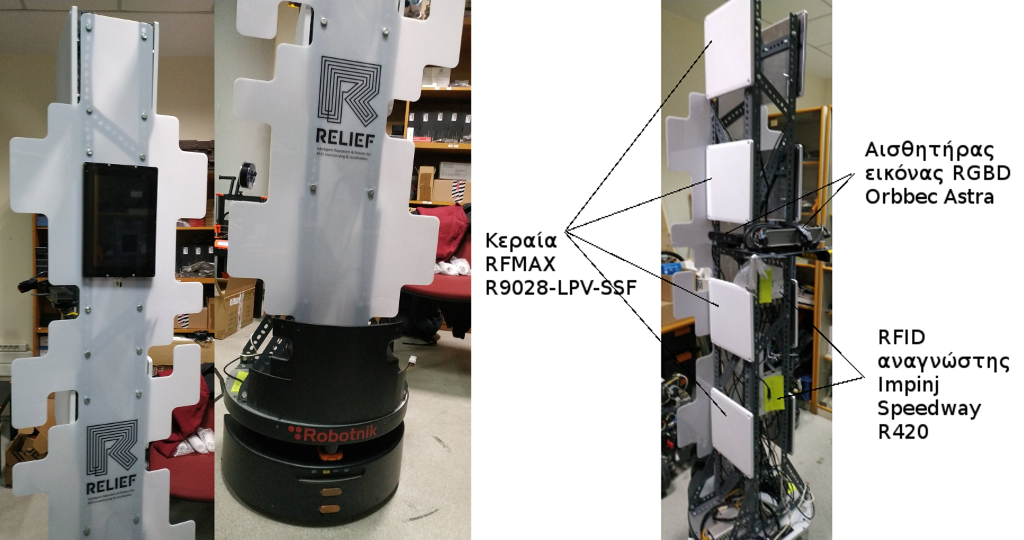
\includegraphics[scale=0.4]{images/relief/rb1/rb1_1x4.png}
  \caption{\small Views of the modified Robotnik RB1 robot used as a heavyweight
           autonomous ground vehicle for inventorying and 3D localisation of
           RFID tags. Source: project deliverable \#9}
  \label{fig:relief_rb1_1x4}
\end{figure}
%\end{minipage}

\begin{figure}[H]\centering
  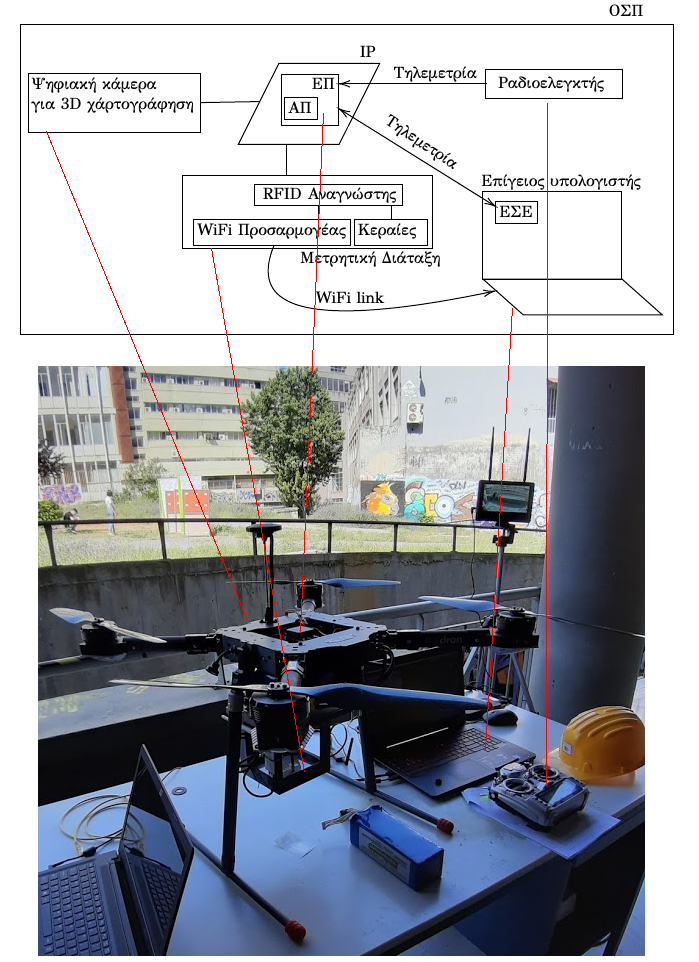
\includegraphics[scale=0.6]{images/relief/drone/drone_arch_corr.png}
  \caption{\small The modified Italdron Evo 4HSE used as an autonomous aerial
           vehicle for inventorying and 3D localisation of RFID tags and the
           architecture of entire flight-and-control system. Source: project
           deliverable \# 12}
  \label{fig:relief_drone}
\end{figure}

%\begin{minipage}[t][\textheight]{\textwidth}
Images \ref{fig:csal_maps} and \ref{fig:e_map} depict (a) a 2D map and (b) a 3D
octomap of the Laboratory of Computer Systems Architecture of the Aristotle
University of Thessaloniki's (AUTh) Department of Electrical and Computer
Engineering, while (c) shows a loose mesh map of the eastern-most corner of
the AUTh campus (\href{https://maps.app.goo.gl/zDzM8HKzkMiFyHMJ6}{40°37'37.7"N
22°57'38.8"E}).

\vfill

\begin{figure}[H]\centering
  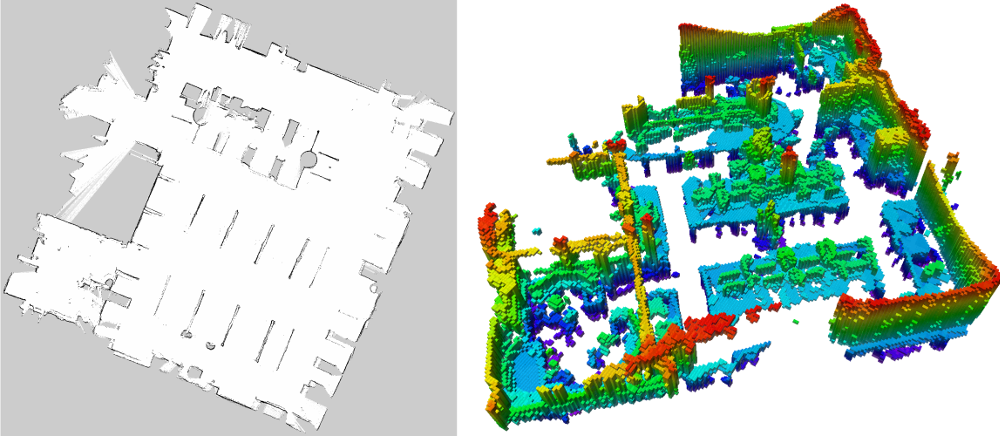
\includegraphics[scale=0.4]{images/relief/csal_maps.png}
  \caption{\small The 2D and 3D map of AUTh's CSAL built by the heavyweight
           autonomous ground robot}
  \label{fig:csal_maps}
\end{figure}

\vfill

\begin{figure}[H]\centering
  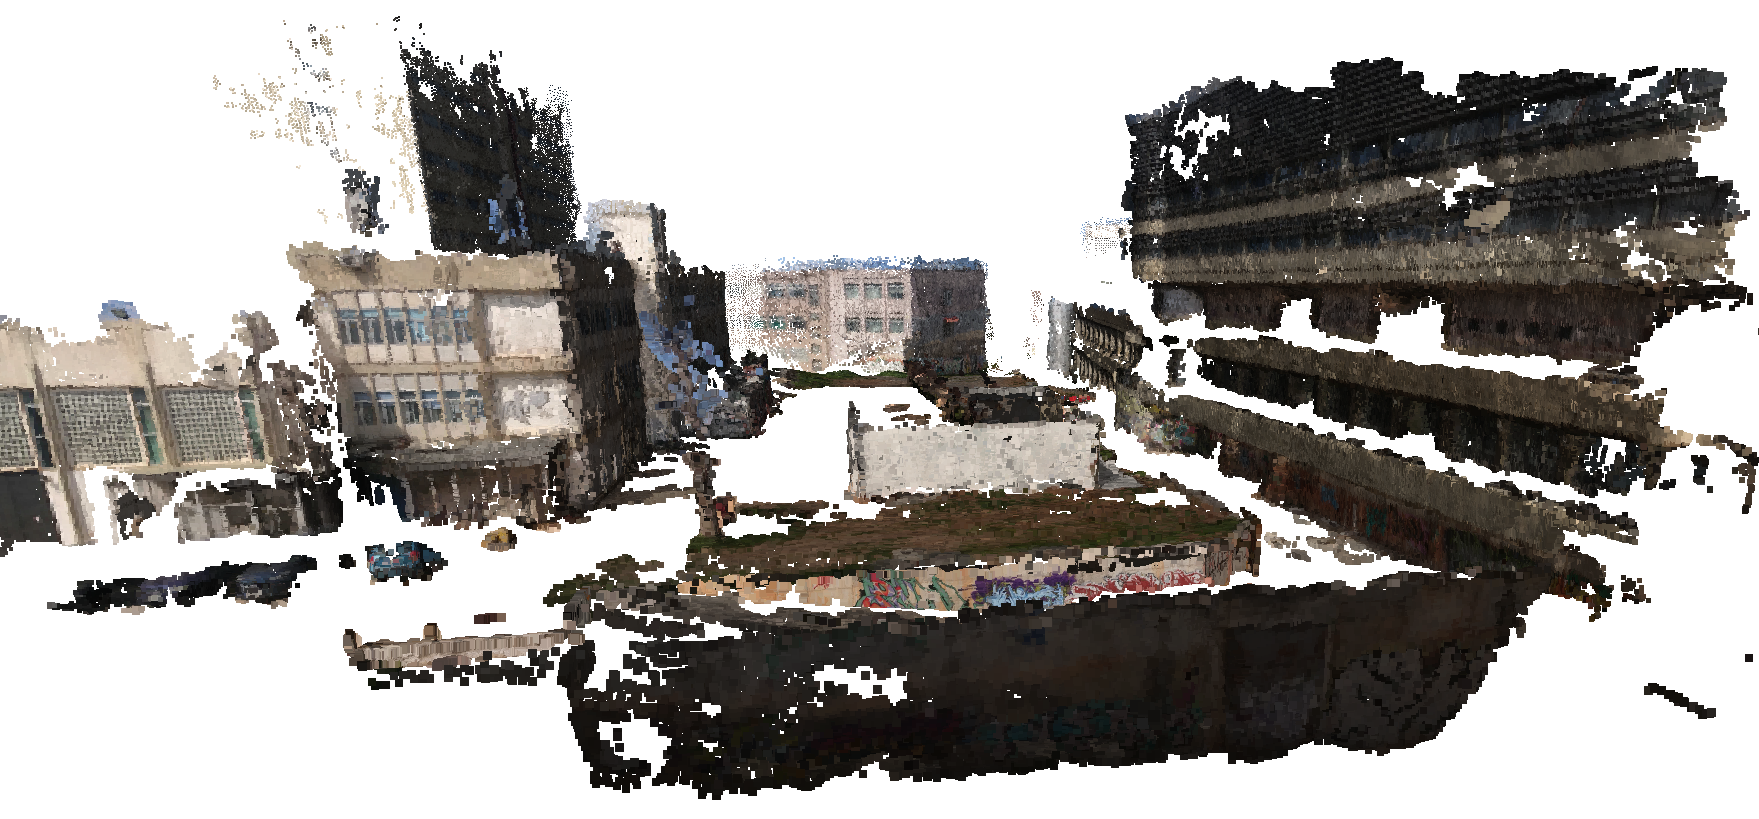
\includegraphics[scale=0.3]{images/relief/e_map.png}
  \caption{\small A mesh map of the outdoor space surrounding AUTh's CSAL,
           built by the autonomous aerial robot}
  \label{fig:e_map}
\end{figure}
%\end{minipage}


%\begin{minipage}[t][\textheight]{\textwidth}
Images \ref{fig:relief_beyond_1} and \ref{fig:relief_beyond_2} show the end
result of autonomous real-time mapping of 3D space for RFID tags by the
project's heavyweight autonomous robot. The demos took place live at the Beyond
Expo in 2021.

%\vfill

%\begin{figure}[H]\centering
  %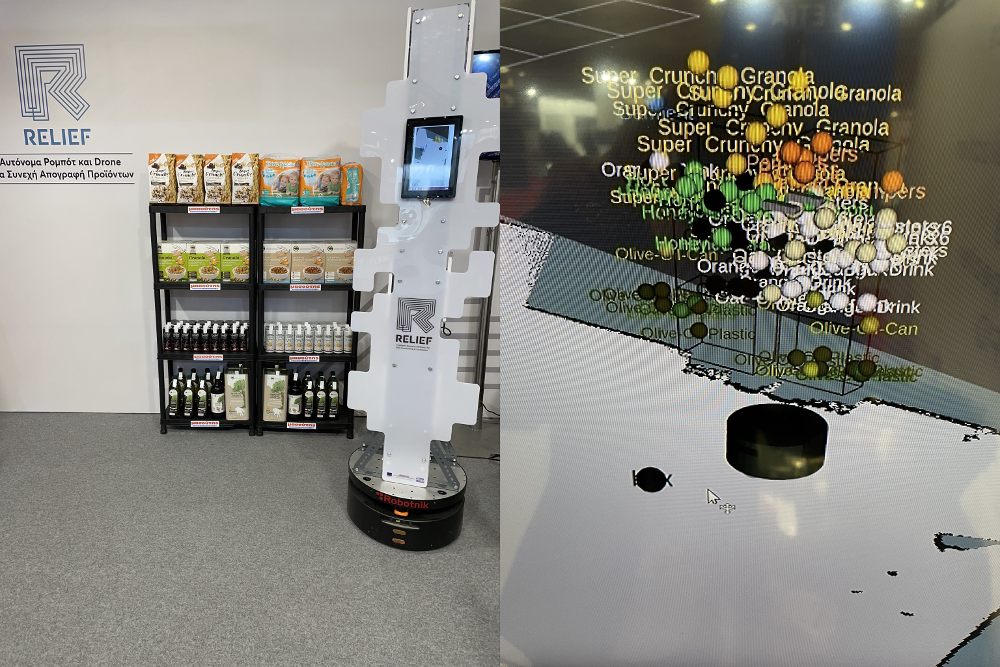
\includegraphics[scale=0.4]{images/relief_1.png}
  %\caption{\small Left: RELIEF's heavyweight autonomous ground vehicle at the
           %Beyond Expo 2021 and a collection of RFID-tagged supermarket
           %products. Right: the robot's perception of the reconstructed map of
           %the products in physical space}
  %\label{fig:relief_beyond_1}
%\end{figure}

%\vfill

\begin{figure}[H]\centering
  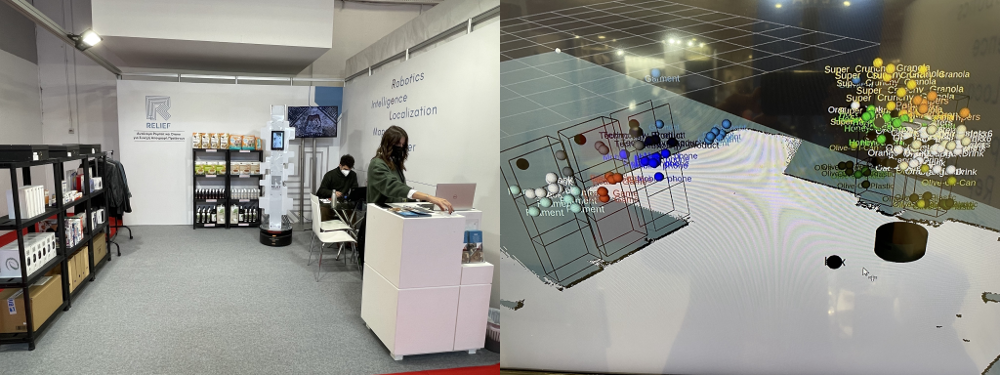
\includegraphics[scale=0.5]{images/relief_2.png}
  \caption{\small The total view of the project's booth wrt image
           \ref{fig:relief_beyond_1}}
  \label{fig:relief_beyond_2}
\end{figure}
%\end{minipage}


You may find an extensive briefing of all of the project's objectives,
applications, advantages and more at its website:
\url{http://relief.web.auth.gr/}.

% TODO GUI


\begin{itemize}
  \item Notions/resources/tools used: \texttt{ROS}, Linux, Hokuyo LIDAR, 2D/3D SLAM, Depth ASTRA Cameras, \texttt{amcl}, \texttt{git}, \texttt{RTAB-Map}, Impinj R420 RFID Reader, Rasa, ReSpeaker Mic Array
  \item Publications resulted from this work: \cite{9617436,Filotheou2022a,FILOTHEOU2023100288,10160120,9981228}
\end{itemize}
